% ****** Start of file apssamp.tex ******
%
%   This file is part of the APS files in the REVTeX 4.1 distribution.
%   Version 4.1r of REVTeX, August 2010
%
%   Copyright (c) 2009, 2010 The American Physical Society.
%
%   See the REVTeX 4 README file for restrictions and more information.
%
% TeX'ing this file requires that you have AMS-LaTeX 2.0 installed
% as well as the rest of the prerequisites for REVTeX 4.1
%
% See the REVTeX 4 README file
% It also requires running BibTeX. The commands are as follows:
%
%  1)  latex aps25samp.tex
%  2)  bibtex apssamp
%  3)  latex apssamp.tex
%  4)  latex apssamp.tex
%
\documentclass[%
 reprint,
nofootinbib,
%superscriptaddress,
%groupedaddress,
%unsortedaddress,
%runinaddress,
%frontmatterverbose,
%preprint,
%showpacs,preprintnumbers,
%nofootinbib,
%nobibnotes,
%bibnotes,
aps,
%pra,
%prb,
%rmp,
%prstab,
%prstper,
%floatfix,
]{revtex4-1}



\usepackage[utf8]{inputenc}
\usepackage[english]{babel}
\usepackage{dsfont}
\usepackage{amsmath}
\usepackage{ mathrsfs }
\usepackage{amssymb}
\usepackage{graphicx}% Include figure files
\usepackage{dcolumn}% Align table columns on decimal point
\usepackage{bm}% bold math
\usepackage{amsmath}
\usepackage{varioref}
\usepackage{booktabs}
\usepackage[bottom]{footmisc}
\usepackage{minted} % for pseudocode

\usepackage{physics}
\usepackage[ruled,vlined]{algorithm2e}
\usepackage{algpseudocode}
\usepackage{listings}

\usepackage{booktabs}

\usepackage{tikz}
\usepackage{float}
\usepackage{siunitx}



\newcolumntype{C}{>{$}c<{$}}
\AtBeginDocument{
\heavyrulewidth=.08em
\lightrulewidth=.05em
\cmidrulewidth=.03em
\belowrulesep=.65ex
\belowbottomsep=0pt
\aboverulesep=.4ex
\abovetopsep=0pt
\cmidrulesep=\doublerulesep
\cmidrulekern=.5em
\defaultaddspace=.5em
}

\usepackage{ntheorem}
\newtheorem{theorem}{Teorem}
\newtheorem*{theorem-non}{Teorem}
\usepackage{hyperref}% add hypertext capabilities
%\usepackage[mathlines]{lineno}% Enable numbering of text and display math
%\linenumbers\relax % Commence numbering lines

%\usepackage[showframe,%Uncomment any one of the following lines to test
%%scale=0.7, marginratio={1:1, 2:3}, ignoreall,% default settings
%%text={7in,10in},centering,
%%margin=1.5in,
%%total={6.5in,8.75in}, top=1.2in, left=0.9in, includefoot,
%%height=10in,a5paper,hmargin={3cm,0.8in},
%]{geometry}

% \renewcommand{\vec}[1]{\mathbf{#1}} %ny definisjon av \vec så det blir bold face i stedet for vector-pil.

\begin{document}


\title{En videnskablig analyse af den maritime tommelfingerregel for vurderingen af kollisionskurs ved betragtning af baggrundens relative bevægelse til et andet fartøj}
\author{Mikkel Metzsch Jensen}

\affiliation{Department of Physics, University of Oslo\\}
\date{\today}


\begin{abstract}
  In this article we investegate the rule of thumb for recognizing when two boats are on a collision course. The proposed statement to be analyzed, namely \textit{The background method}, can be formulated briefly as: "If the static background seen behind the oncoming boat does not visually move relatively to the boat, then you are on a collision course.". The analysis have shown that this statement is strongly related to the dertermination of the relative bearing. By mathematical proof we found that if and only if two boats, with constant velocity which approaches each other in distance, have constant relative bearing they are on collision couse. Therefore the determination of the relative bearing is the most precise way of recognizing a collision course. On the other hand we found that the background method can be used as a means to determine whether the relative bearing is constant in special cases. This were mainly derived by an analytical approach but is also supported by numerical simmulations. In general the background method is found to be valid when used in greater distances to the coast, losely estimated to approximately 833 meters or more (safe distance to use). The exact estimat builds on the velocity of the observer, the tolerance definition for a humanly recognizable angular velcoty and is dependent on the value of the relative bearning and the angle between the heading and the coast. The nature of this relationship is showcased on figure \ref{fig:limit_dimension} and \ref{fig:limit_coastdis}.
\end{abstract}


\maketitle



\section{Introduktion}
Som søfarer findes der en række nødvendige og basale regler som sikrer god orden og sikkerhed til søs. Heriblandt har vi vigereglerne, som regulerer færdslen på vandet og forebygger, at skibe støder sammen \cite{respektforvand}. Disse regler beskriver som udgangspunkt, hvordan man skal agere, hvis man er på kollisionskurs med andre fartøjer. Det er naturligvis fordelagtigt for søfaren at blive opmærksom på en sådan kollisionfare i så god tid som mulig, så man kan korrigere kurs eller fart. \par
Denne rapport udsprigner af en diskussion med Lars Juel Hansen (sommeren 2019) om en tommelfingerregel for netop vurderingen af kollisionskurs. Denne tommelfingerregel består af en metode, hvorpå iagttageren bruger baggrunden som referanse til at afgøre om man er på kollisionskurs eller ikke. Vi skal fremadrettet kalde den metode for \textit{baggrundsmetoden}, og den formuleres her som følger.
\begin{quote}
\textbf{Baggrundsmetoden}: Betragt båden som du mistænker en mulig kollision med, og noter et fastliggnede punkt i baggrunden som synes akkurat bag båden. Hvis dette baggrundspunkt i den efterfølgende observationsperiode lader til at flytte sig i forhold til båden, da er du \underline{ikke} på kollisionskurs med båden. Forbliver baggrundspunktet derimod i sigtelinjen bag båden er dette en indikator på at kollisionskursen er reel.
\end{quote}
Ved en undersøgelse af tilgængelige internetkilder findes forskellige gengivelser af denne regel. Ifølge Duelighed.dk \cite{duelighed} kan man ved "betydelige afstande" til kysten bruge observationen om hvordan kollisionsfartøjet trækker "over land" til at vurdere pejlingen til kollisionsfartøjet. Pejlingen er retning fra iagttageren til den genstand, der pejles \cite{ordbog}, og der hævdes i denne sammenhæng:
\begin{quote}
   "[...] fare skal anses for at være til stede, hvis pejlingen af et skib, der nærmer sig, ikke kendeligt forandrer sig." - Duelighed.dk \cite{duelighed}
\end{quote}
Således siger reglen, hvis den modsejlende trækker mod styrbord i forhold til baggrunden, så vil fartøjet gå styrbord om iagttagerens fartøj. Modsat vil det gå bagbord om iagttagerens fartøj, hvis det trækker til bagbord over land. Hvis ikke fartøjet bevæger sig kendeligt i forhold til baggrunden, vil det indikere at fartøjerne er på kollisionskurs. \par
Dette er i overenstemmelse med baggrundsmetoden, som vi ønsker at undersøge. Dog er det værd at bemærke at metoden fra Duelighed.dk indføres som et middel til at vurdere om der er pejltræk (om pejlingen til kollisionsfartøjet ændres). \par
I andre kilder (\cite{studienoter}, \cite{retsinformation} \cite{groensund}) er det netop pejlingen, som angives som den direkte indikator på kollisionskurs. Her henvises til en mere direkte fremgangsmåde for at vurdere om der er pejltræk, ved at anvende et fastliggende punkt på eget fartøj som referanse.  Vi vil fremadrettet betegne denne metode som \textit{lokalpunktsmetoden}, og den formuleres her som følger.
\begin{quote}
\textbf{Lokalpunktsmetoden}: Betragt båden som du mistænker en mulig kollision med, og noter et fastliggnede punkt på eget fartøj (f.eks. et punkt på rælingen), som synes i sigtelinjen til båden. Hvis båden i den efterfølgende observationsperiode lader til at flytte sig i forhold til punktet, da er der pejltræk, og du er \underline{ikke} på kollisionskurs med båden. Forbliver båden derimod i sigtelinjen fra punktet er dette en indikator på, at der ikke er pejltræk og at kollisionskursen er reel.
\end{quote}
Der fremstår nu to centrale spørgsmål for vurderingen af baggrundsmetodens pålidelighed:
\begin{enumerate}
  \item Hvilken sammenhæng findes der mellem pejltræk til en anden båd og en mulig kollisionskurs.
  \item I hvilken grad kan baggrundsmetoden bruges til at vudere om der er pejltræk.
\end{enumerate}
I denne rapport skal vi fremføre en matematisk analyse af baggrundsmetodens pålidelighed ved at behandle de to overstående spørgsmål. \par
Rapporten bestræber sig på at give en fyldestgørende beskrivelse af det omtalte problem, samtidig som at dette formidles til en målgruppe uden særlig matematisk baggrund. Dette er ikke mulig på alle punkter, da en ordenlig bevisførelse kræver en hvis mængde matematik. Jeg har dog forsøgt at gengive de underliggende resultater og vigtiste pointer undervejs, således at man kan springe beregninger og udledninger over uden at miste kontekst. Dette gælder særlig udledningen i afsnit \ref{sec:pejling_betydning}.


\section{Metode}
\subsection{Definering af problemet}
Vi forestiller os to både til søs, som nærmer sig hinanden. Vi kalder den ene båd for hovedbåden (HB), hvor vi har placeret iagttageren, og den anden båd kalder vi for kollisionsbåden (KB). Vi antager at begge bådene bevæger sig med konstant hastighed, dvs. retlinjet og med konstant fart. Vi beskriver hver båd som et enkelt punkt i et koordinatsystem med akserne $x$ og $y$ som angiver bådens position på vandets overflade set oppefra (se figur \ref{fig:metode_tegning}). Hvis vi kender startpositionen og hastigheden til hver båd, har vi alt den information vi trænger for at beskrive situationen. \par Formelt set kan vi beskrive position $\vec{P} = (x, y)$ som en funktion af tid $t$, når vi kender startposition $\vec{P}_0$ og hastighed $\vec{v}$. For de to både har vi dermed bevægelseslingingen
\begin{align}
  \vec{P}(t) =  \vec{P}_0 + \vec{v}\cdot t
  \label{eq:motion}
\end{align}
Hvis du allerede nu føler en ubehag i kroppen ved synet af ligniner og andre matematiske redskaber, så vil jeg understrege at det holder at tænke på dette som en oversættelse fra ord til tal. Det vigtiste at forstå her, er at vi beskriver bådene som punkter i et koordinatsystem, som bevæger sig i rette linjer med uændret hastighed. \par
Vi definerer en kollision som tilfældet hvor bådene har samme position til samme tidspunkt. I praksis vil man have en kollision allerede hvis bådende passerer tæt forbi hinanden, da bådene naturligvis har en hvis udstrækning. Dette er dog en unødvendig detalje at medregne for dette problem, og vi kan derfor trygt fortsætte at tænke på bådene som enkelte punkter. For at vudere om bådene er på kollisionskurs, er det angiveligt nyttigt at benytte pejlingen. Vi definerer i matematisk forstand pejlingen $\theta_{HB}$ fra HB til KB som vinklen mellem kursen til HB og sigtelinjen fra HB til KB. Dette er illustreret på figur \ref{fig:metode_tegning}.

\begin{figure}[H]
  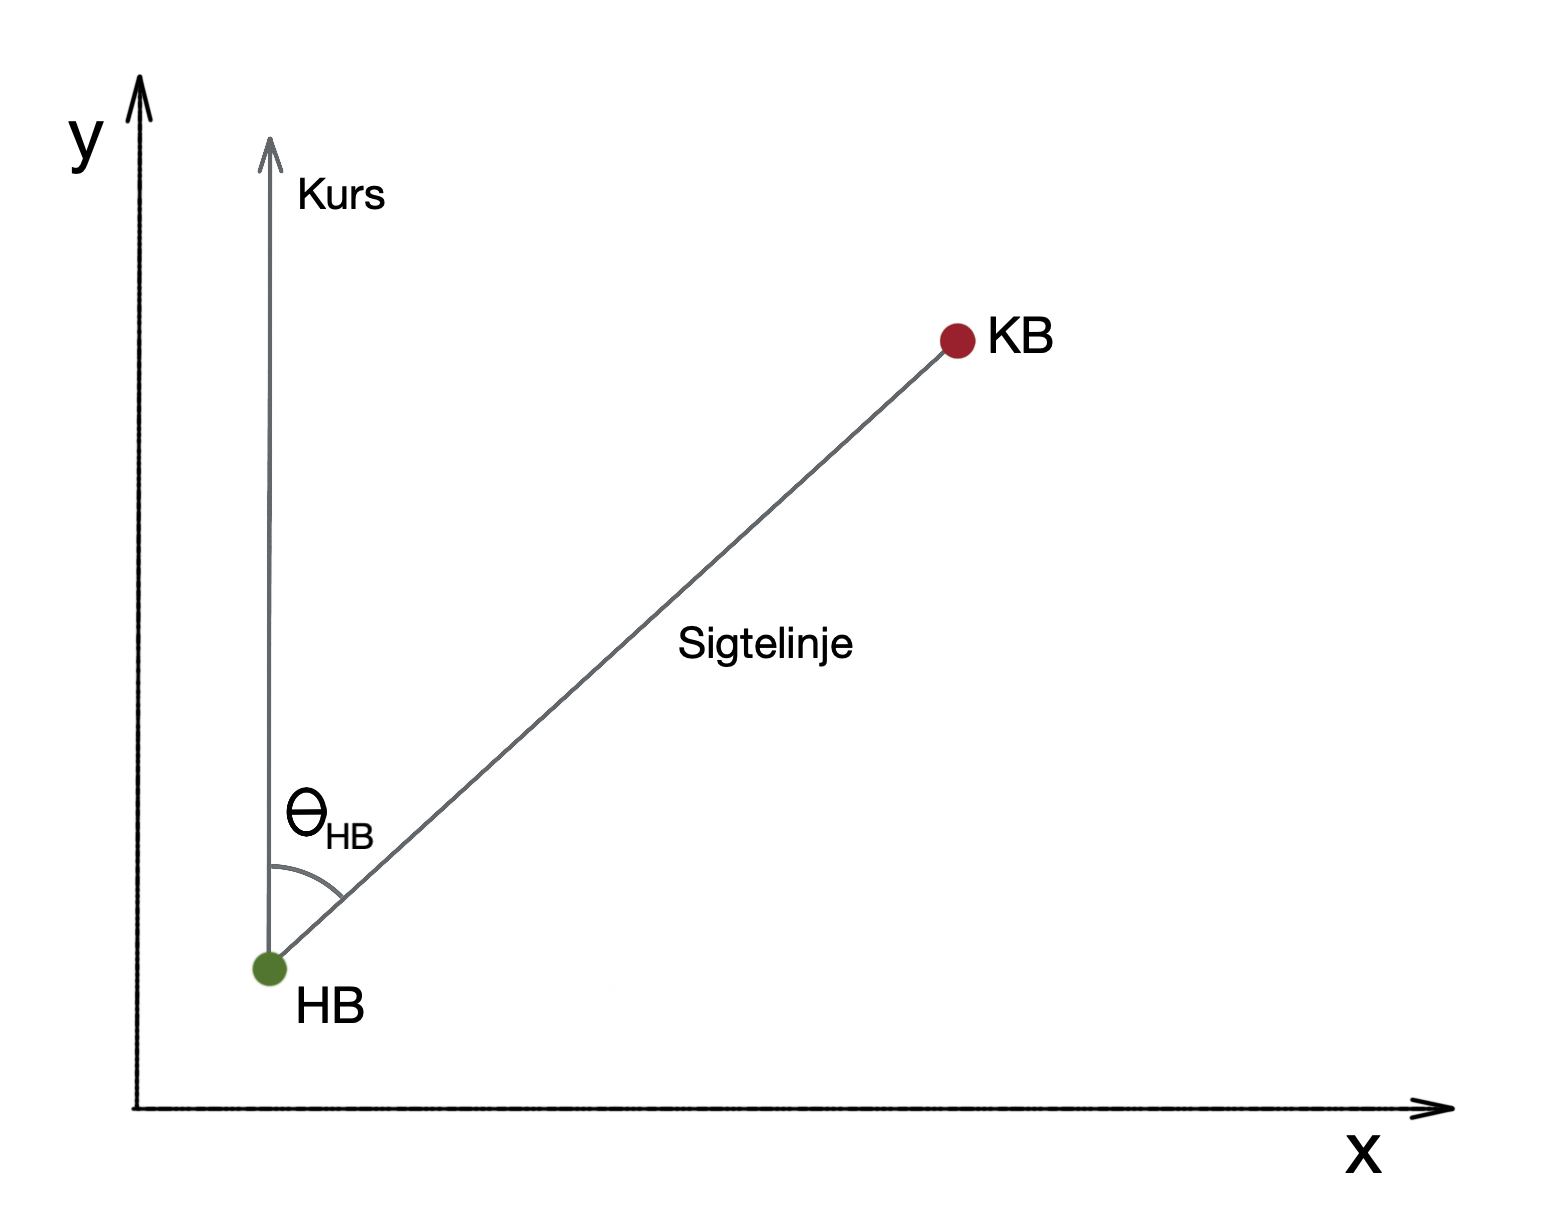
\includegraphics[width=\linewidth]{figures/metode_tegning.png}
  \caption{En illustration af koordinatsystem som beskriver positionen til de to både på vandoverfladen (set fra oven). Her har vi indtegnet pejlingen $\theta_{HB}$ som defineres som vinklen mellem kursen til HB og sigtelinjen fra HB til KB.}
  \label{fig:metode_tegning}
\end{figure}
Ud fra disse definitioner og indførelselen af et koordinatsystem, er vi klar til at give os i kast med en analyse af situationen under forskellige betingelser.

\subsection{Numeriske simuleringer som støtte til matematiske resultater}\label{sec:numerical_method}
I tillæg til den matematiske analyse, skal vi bruge en numeriske metoder (måske bedre kendt som simmuleringer) til støtte af vores resultater. \par
For den interesserede kan vi simmulere bådens præcise bevægelse (uden usikkerhed), da alle bevægelserne er lineære. Dette gøres ved at evaluere bevægelsesligning \ref{eq:motion} ved forskellige tidspunkter, analogt til Eulers metode uden acceleration. Vi skriver simmuleringskoden i python som angivet nedenfor. Denne er også tilgængelig på github \cite{github} sammen med diverse scripts for plotting af data.

\begin{minted}[breaklines, breakautoindent = true]{python}
import numpy as np

def simulator(MB_start, OB_start, MB_end, OB_end, T = 10, dt = 0.1):
    K = int(T/dt + 1)         #Steps
    MB_pos = np.zeros((K,2))  #MB = Main Boat
    OB_pos = np.zeros((K,2))  #OB = Other Boat
    t = np.zeros(K)           #Time

    #Initial position
    MB_pos[0] = MB_start
    OB_pos[0] = OB_start

    #Calculate constant velocity
    MB_vel = (MB_end - MB_pos[0])/T
    OB_vel = (OB_end - OB_pos[0])/T

    #Main update loop
    for k in range(K - 1):
        MB_pos[k+1] = MB_pos[k] + MB_vel*dt
        OB_pos[k+1] = OB_pos[k] + OB_vel*dt
        t[k+1] = t[k] + dt
    return MB_pos, OB_pos
\end{minted}


\section{Resultater}
\subsection{Sammenhæng mellem pejltræk og kollisionskurs}
Vi begynder med en intuitiv forklaring på hvorfor pejltrækket har en helt særlig sammenhæng til kollisjonskursen. For at indse denne sammenhæng skal vi bruge at begge bådende antages at bevæge sig med konstant fart og i en ret linje. Dette har den særlige egenskab at en iagttager på HB også vil se at KB bevæger sig med konstant fart og i en ret linje relativt til iagtagerens perspektiv. Når vi skifter perspektiv siger vi at vi skifter koordinatsystem eller mere formelt intertialsystem. Mens koordinaterne $(x, y)$ angiver positionen på vandet ligesom GPS, så kan vi skifte til koordinatsystemet med koordinaterne $(x',y')$ som angiver position relativt til HB. I dette koordinatsystem vil HB altid være placeret i $(0,0)$ og de andre både beskrives relativt til HB. Det betyder at hvis HB bevæger sig fremad i $(x,y)$-systemet så vil stillestående punkter angives som om at de bevæger bagud i $(x',y')$-systemet. På figur \ref{fig:reference_frame_explainer} ses hvordan koordinaterne til en række bådruter angives i det normale $(x,y)$-system og $(x',y')$-system.

\begin{figure}[H]
  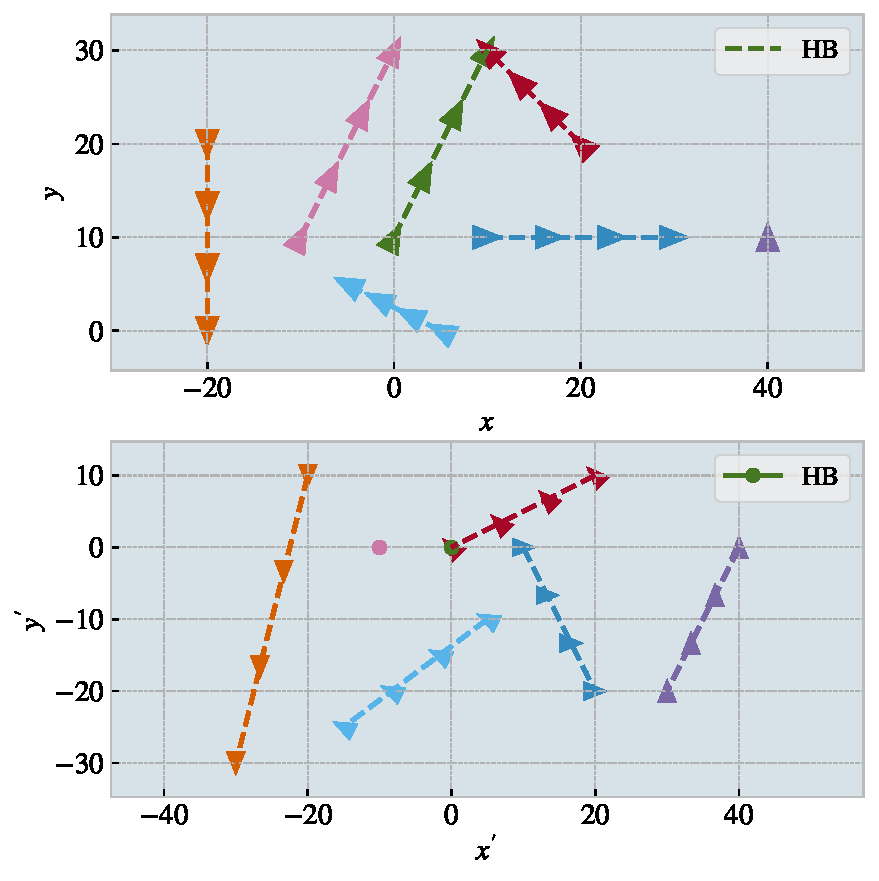
\includegraphics[width=\linewidth]{figures/reference_frame_explainer.pdf}
  \caption{En illustration af ændringen fra koordinatsystemet $(x,y)$ til HB's intertialsystem med koordinaterne  $(x',y')$ for en række vilkårlige bådruter. Bemærk at pilens retning angiver bådens kurs og vi ser i $(x',y')$-system at bådene ser ud til at sejle en smule sidelæns da en del af bevægelsen skyldes at HB selv flytter sig. Bemærk for eksempel at den lille båd som egentlig står stille i $(x,y)$ nu bevæger sig i  $(x',y')$. Tilsvarende står den lyserøde båd i ro i $(x',y')$ fordi den bevæger sig parallelt (og med samme hastighed) som HB. }
  \label{fig:reference_frame_explainer}
\end{figure}

Vi ser altså på figur \ref{fig:reference_frame_explainer} at alle bådende også bevæger sig retlinjet $(x',y')$-systemet. Dermed ved vi at i tilfældet hvor bådene er på kollisionskurs vil en iagttager på HB nødvendigvis se at KB bevæger sig direkte mod iagtageren. Dette er den eneste mulige rette linje hvorpå bådene kan kollidere uden at medparterne ændrer retning eller fart undervejs. Derfor følger det at pejlingen også vil være konstant i tilfældet med kollisionskurs - altså vil en iagtager ikke opleve pejltræk for kollisionsbåden. De eneste andre situationer hvor pejlingen er konstant er når bådene begge ligger stille, sejler parallelt eller sejler væk fra hinanden i modsat retning af kollisionskursen. For disse tre tilfælde nærmer bådene sig ikke i afstand, og det er dermed enkelt at afgøre, at der ikke er kollisionsfare i disse tilfælde. \par
I det følgende afsnit gives en matematisk udledning for dette koncept, som leder ud i en matematisk sætning. Hvis du ikke er til matematik så burde den overstående forklaring være mere end rigelig til at acceptere dette (se teorem \ref{Teo:pejling}).



\subsection{Sammenhæng mellem pejltræk og kollisionskurs (matematisk udledning)}\label{sec:pejling_betydning}
Da vi har antaget at bådene bevæger sig med konstant hastighed, kan vi bruge en lineær transformation til at skifte koordinatsystem til intertialsystemet (dvs. det koordinatsystem som beskriver relativ bevægelse til iagttageren) hvor HB er i ro. Vi kalder dette for HB's intertialsystem. Med andre ord så kan vi frit vælge at beskrive positionen til KB som den opleves for en iagttager ombord på HB. Positionen $\vec{P}'_{KB}$ til KB i det nye intertialsystem kan skrives:
\begin{align*}
  \vec{P'}_{KB}(t) &= \vec{P}_{KB}(t) - \vec{P}_{HB}(t) \\
  &= \vec{P}_{0,KB} + \vec{v}_{KB}t - \vec{P}_{0,HB} - \vec{v}_{HB}t \\
  &= (\vec{P}_{0,KB} - \vec{P}_{0,HB}) + (\vec{v}_{KB} - \vec{v}_{HB})t \\
  &= \vec{P'}_{0,KB} + \vec{v'}_{KB}t
\end{align*}
Vi ser at $\vec{P}'_{KB}$ også beskriver en retlinjet bevægelse. I tilfældet hvor bådene er på kollisionskurs ved vi at $\vec{P}'_{KB}(t_k) = \vec{0}$ ved kollisionstidspunktet $t_{k}$. Dette medfører sammenhængen:
\begin{align}
  \vec{P'}_{0,KB} &= - \vec{v'}_{KB}t_k \nonumber \\
  \begin{pmatrix} x'_{0,KB} \\ y'_{0,KB} \end{pmatrix}\frac{1}{t_k} &=   -\begin{pmatrix} v'_{x,KB} \\ v'_{y,KB} \end{pmatrix}
  \label{eq:P=v}
\end{align}
Vi kan da finde pejlingen $\theta_{HB}$ ved at omrksive $\vec{P}'_{KB}$ til polære koordinater. Her er vi bare interesseret i vinkelkoordinat $\phi_{KB}$ som kan bestemmes som
\begin{align*}
  \phi_{KB}(t) &= \arctan{\left( \frac{y'(t)}{x'(t)}\right)} \\
  &= \arctan{\left( \frac{y'_{0,KB} + v'_{y,KB}t}{x'_{0,KB} + v'_{x,KB}t}\right)}
\end{align*}
Vi bruger da sammenghængen fra ligning \ref{eq:P=v} og finder
\begin{align*}
  \phi_{KB}(t) &= \arctan{\left( \frac{y'_{0,KB} - y'_{0,KB}\frac{t}{t_k}}{x'_{0,KB} - x'_{0,KB}\frac{t}{t_k}}\right)} \\
  &= \arctan{\left(\frac{y'_{0,KB}}{x'_{0,KB}} \frac{1 - \frac{t}{t_k}}{1 - \frac{t}{t_k}}\right)} \\
  &= \arctan{\left(\frac{y'_{0,KB}}{x'_{0,KB}}\right)} = \text{konst.} \\
\end{align*}
Fra dette ser vi at vinkelkoordinat $\phi_{KB}$ er konstant (uavhængig af tid), hvilket medfører at pejlingen også er konstant:
\begin{align*}
  \theta_{HB} &= \frac{\pi}{2} - \phi_{KB} = \text{konst.}
\end{align*}
Fra dette ræsonoment har vi altså vist at pejlingen vil være konstant i tilfældet hvor bådene er på kollisionkurs. Hvis bådene følger kollisionskursen men i modsat retning (bevæger sig væk fra hianden), kan vi indføre betingelsen $\vec{P}'_{KB}(t_i) = \vec{0}$ for et tidspunkt $t_i < 0$. Derved kan vi opstille en ligning tilsvarende \ref{eq:P=v} og derved finde at pejlingen også vil være konstant i dette tilfælde. Hvis ikke bådene er på kollisionskurs er ligning \ref{eq:P=v} ikke længere gyldig og $P'_{KB}$ kan tage hvilken som helst retlinjet bane uden om $\vec{P}'_{KB} = \vec{0}$. Det betyder at $\phi_{KB}$ og dermed også pejlingen $\theta_{KB}$ vil ændre sig som funktion af tid. Dette fører til slutningen:
\begin{theorem}
  Hvis og bare hvis to både med konstant hastighed som nærmer sig i afstand har konstant pejling til hinanden er disse på kollisionskurs.
  \label{Teo:pejling}
\end{theorem}


\subsection{Grænsebetingelser for brug af baggrundsmetoden}
Med udgangspunkt i teorem \ref{Teo:pejling} kan vi undersøge om brugen af baggrundensmetoden er en pålidelig indikator for en fremtidig kollision.
Vi skal altså undersøge om der er sammenfald mellem en konstant pejling og tilfældet hvor baggrunden ikke bevæger sig relativt til sigtelinjen gennem KB. \par
I tilfældet med kollisionskurs ved vi fra teorem \ref{Teo:pejling} at sigtelinjen fra HB gennem KB vil have en konstant vinkel. I det enkle tilfælde hvor kystlinjen er relinjet og parallel med kursen til HB vil sigtelinjens skæring med kystlinjen forflytte sig med samme hastighed som HB. Dette resultat bekræftes ved simuleringen vist på figur \ref{fig:eks1}.
\begin{figure}[H]
 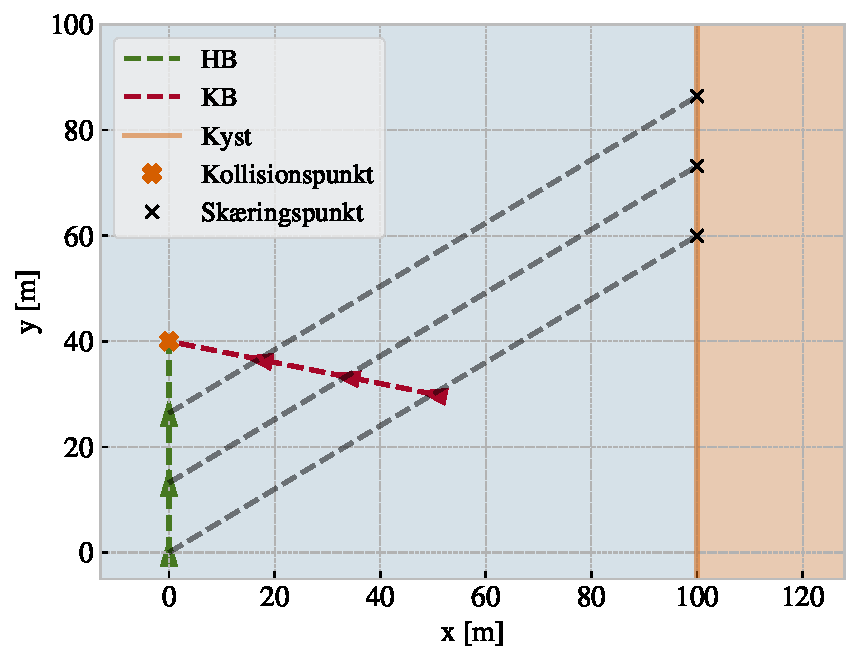
\includegraphics[width=\linewidth]{figures/eksempel1.pdf}
 \caption{En simulering af bådene HB og KB på kollisionskurs, med kollisionspunkt 100 meter fra kysten. Her plottes fire positioner for bådene (inklusiv kollisionspunktet) jævnt fordelt i tid. Fra de grå stiblede linjer ser vi hvordan sigtelinjen fra HB gennem KB skærer med kysten. Dette skæringspunkt forflytter sig som forventet i henhold til HB's bevægelse.}
 \label{fig:eks1}
\end{figure}
 Hvis sigtelinjens skæring med kystlinjen forflytter sig kendelig, på trods af at bådene er på kollisionskurs (pejlingen er konstant), vil baggrundsmetoden være vildledene. Vi undersøger derfor hvordan afstanden til kysten spiller en rolle for hvorvidt forflytningen er kendelig. \par
 Fra HB's perspektiv vil baggrundspunktet (BP) bevæge sig med en hastighed $\vec{v'}_{BP} = - \vec{v}_{HB}$. Dette giver en observeret vinkelhastighed $\omega_O$:
 \begin{align*}
   \omega_O = -\frac{v_{HB}\sin{(\theta_{HB})}}{d}
 \end{align*}
 hvor $v_{HB} = |\vec{v}_{HB}|$ er bådens fart, $\theta_{HB}$ er pejlingen og $d$ er afstanden til kysten via sigtelinjen. Hvis vi definerer minimumsgrænsen for en kendelig forflytning som vinkelhastigheden $\omega_k$ får vi at kriteriet for anvendelse af baggrundsmetoden er
 \begin{align}
   |\omega_O| &< \omega_k \nonumber \\
   \frac{v_{HB}\sin{(\theta_{HB})}}{d} &< \omega_k \nonumber \\
   \frac{v_{HB}\sin{(\theta_{HB})}}{\omega_k} &< d
   \label{eq:limit}
 \end{align}
Vi kan da bruge denne sammenhæng til at finde den minimale afstand $d$ for brug af baggrundsmetoden som funktion af $\theta_{HB}$. Dette resultat er vist på figur \ref{fig:limit_dimensionless}.
 \begin{figure}[H]
   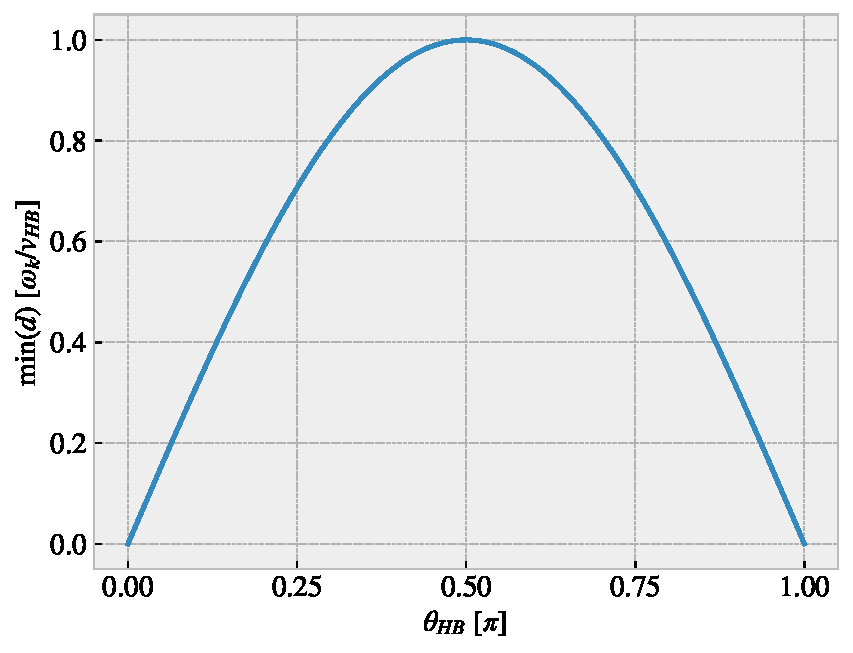
\includegraphics[width=\linewidth]{figures/limit_dimensionless.pdf}
   \caption{Den minimale afstand $\min{(d)}$ som funktion af pejlingen $\theta_{HB}$ som mulliggør brug af baggrundsmetoden. $d$ beskriver afstanden til kysten via sigtelinjen. Resultatet er angivet med dimensionløse enheder med skaleringsfaktorene $\omega_k$ som er den minimumme vinkelhastighed for en kendelig forflytning og $v_{HB}$ som er farten til HB. For at baggrundsmetoden skal være anvendelig, må vi kræve at $d$ ligger over kurven for $\min{(d)}$.}
   \label{fig:limit_dimensionless}
 \end{figure}


\subsubsection{Definering af kendelig forflyting}
For at bestemme enhederne til figur \ref{fig:limit_dimensionless}, må vi definere hvad en kendelig forflytning er. Hertil bruger vi en række kvalificerede gæt for at finde et estimat for $\omega_k$. Bemærk at følgende resultater derfor bygger på en del usikkerheder. \par
Vi kan forestille os at vi ved observation af KB vil benytte et centralt punkt på båden som referanse mod baggrunden. En mulig defintion på en kendelig forflytning kan da være at baggrundspunktet har flyttet sig ud til eller forbi kanten af båden i løbet af en observationsperiode. Observationsperioden estimeres til 10 sekunder, svarende til den nedre grænse af tidsintervallet 10-20 sekunder som nævnes i \cite{duelighed}. Vi siger da at forflytningen er kendelig hvis baggrundspunktet har flyttet sig en relativ afstand større eller lig halvdelen af bådens tværlængde set fra iagttageren i løbet af de 10 sekunder. For sejlbåde i den lidt større klasse kan vi bruge en gennemsnitlig bredde på 5 m og længde på 15 m, hvilket giver 10 m som middelestimat (tilsvarer 45 graders sigtelinje). Til sidst må vi vudere den afstand der er mellem to skibe når kollisionsrisikoen vurderes. Hertil bruges 200 meter som en minimumsværdi. Ud fra dette finder vi at en kendelig forflytning kan defineres ved en vinkelhastighed større eller lig $\omega_k$:
\begin{align}
  \omega_k = \frac{\arctan{(\frac{1}{2}\frac{10 \text{m}}{200 \text{m}})}}{10 \text{s}} = 0.0025 s^{-1} \approx  0.14^{\circ}s^{-1}
  \label{eq:omega_k}
\end{align}
Bemærk at disse antagelser udelukkende gøres for estimere menneskets evne til at kende en forflytning i praksis. Hvis værdien for menneskets evne til at kende en forflytning hentes fra faktiske studier vil det være at foretrække. Ved valg af den nedre grænse for observationsperioden, et stort estimat for bådens tværlængde og et minimumsestimat for afstanden mellem bådene ved observation, estimerer vi effektivt den øvre grænse for en kendelig forflytning. Dette vil føre til at estimatet for den gyldige afstand $d$ bliver et minimumsestimat og dermed giver de bedste vilkår for baggrundsmetodens gyldighed. \par
Vi kan nu bruge at en typisk bådhastighed er 4 knob hvilket tilsvarer omtrent 2 m/s. Med disse værdier kan vi skalere resultatet fra figur \ref{fig:limit_dimensionless} sådan at vi får enhederne vist på figur \ref{fig:limit_dimension}.
\begin{figure}[H]
  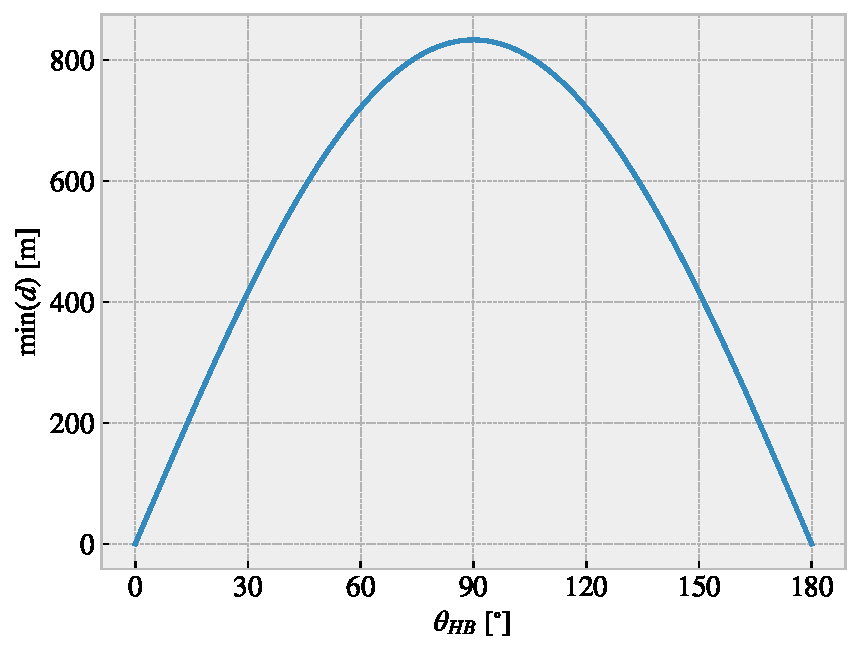
\includegraphics[width=\linewidth]{figures/limit_dimension.pdf}
  \caption{Den minimale afstand $\min{(d)}$ som funktion af pejlingen $\theta_{HB}$ som mulliggør brug af baggrundsmetoden. $d$ beskriver afstanden til kysten via sigtelinjen i meter. Enhederne er fastlagt ud fra figur \ref{fig:limit_dimension} med brug af estimater for $\omega_k$ og $v_{HB}$.}
  \label{fig:limit_dimension}
\end{figure}
I en situation hvor den retlinjede kyst har en vinkel $\beta$ i forhold til HB's kurs kan vi omregne afstanden $d$ langs sigtelinjen til den korteste afstand $s_{kyst}$ mellem HB og kysten (linjen vinkelretpå kysten). Omregning gøres som
\begin{align}
  s = d\cdot \sin{(\theta_{HB} + \beta)}
  \label{eq:s_kyst}
\end{align}
Ved at anvende denne omregning får vi resultatet vist på figur \ref{fig:limit_coastdis}.
\begin{figure}[H]
  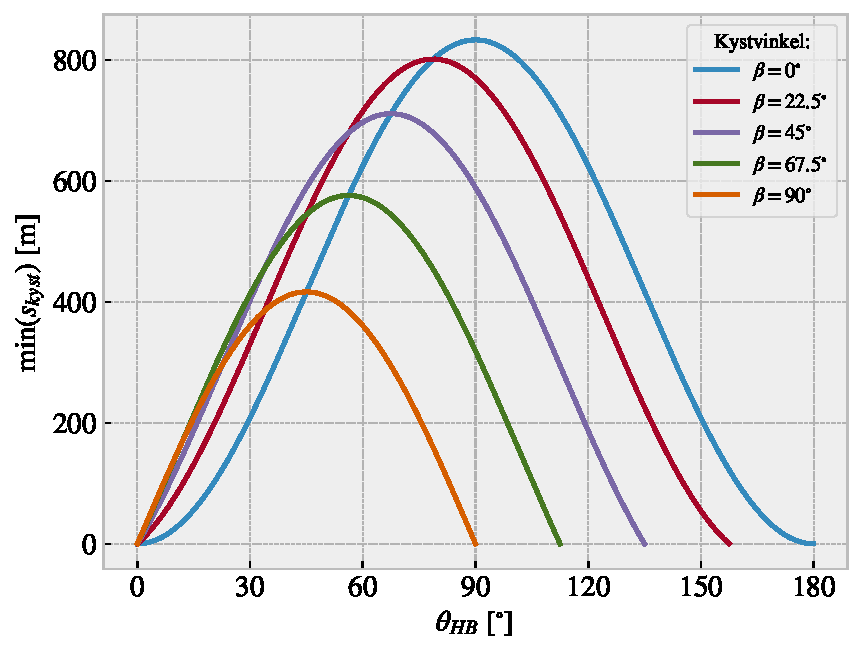
\includegraphics[width=\linewidth]{figures/limit_coastdis.pdf}
  \caption{Den minimale afstand $\min{(s_{kyst})}$ som funktion af pejlingen $\theta_{HB}$ som mulliggør brug af baggrundsmetoden. $s_{kyst}$ (se ligning \ref{eq:s_kyst}) er den korteste afstand for HB til kysten, når kysten har en vinkel $\beta$ i forhold til HB's kurs.}
  \label{fig:limit_coastdis}
\end{figure}

Da det er upraktisk at skulle vurdere vinklen til kysten kan vi forsimple dette resultat lidt. Vi ser på \ref{fig:limit_coastdis} at når $\beta$ øger fra 0 til 90$^{\circ}$ så forskydes den grunnlæggende kurve for $\beta = 0$ samtidig som at den formindskes. Vi er nu interesseret i at finde en kurve som indeholder alle disse forskydninger fra variation af $\beta$, således at vi har en effektiv maksimumskurve for $\min{(s_{kyst})}$. Dette tilsvarer at vi tager den maksimale værdi for $\min{(s_{kyst})}$ i hvert punkt ved at vælge den kystvinkel $\beta$ som giver den største værdi. Vi husker at
\begin{align*}
  s_{kyst} \propto \sin{(\theta_{HB} + \beta)}
\end{align*}
og derved ser vi at vi opnår maksimalværdi ved at vælge $\beta = \frac{\pi}{2} - \theta_{HB}$. Da finder vi at den maksimale værdi som funktion af $\theta_{HB}$ er
\begin{align}
  \max{(s_{kyst})}(\theta_{HB}) = d
  \label{eq:max_s_kyst}
\end{align}
Bruger vi denne approksimation får vi et anvendelig plot for aflæsning af den gyldige zone for baggrundsmetoden uavhængig af kystvinklen. Dette er vist på figur \ref{fig:limit_coastdis_betamax}.
\begin{figure}[H]
  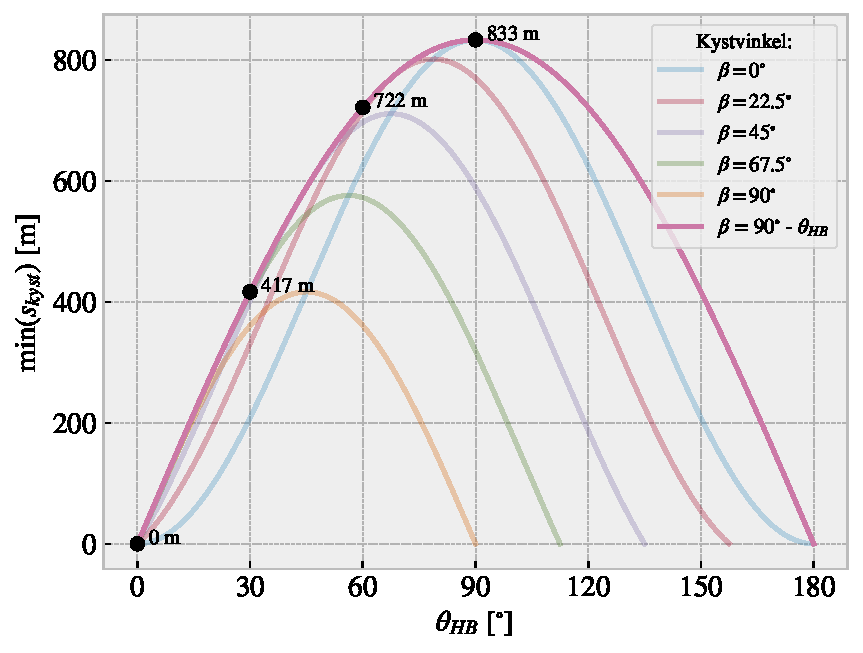
\includegraphics[width=\linewidth]{figures/limit_coastdis_betamax.pdf}
  \caption{Den minimumme afstand $\min{(s_{kyst})}$ som funktion af pejlingen $\theta_{HB}$ som muliggør brug af baggrundsmetoden (se figur \ref{fig:limit_coastdis}). Den lyserøde kurve for $\beta = 90^{\circ} - \theta_{HB}$, tilsvarerer det valg af $\beta$ for hvert punkt som giver den største værdi. Dermed har vi et maksimumsestimat på $\min{(s_{kyst})}$ som kan aflæses uavhængig af kystvinkel $\beta$ }
  \label{fig:limit_coastdis_betamax}
\end{figure}

\subsection{Numeriske simuleringer}
Ved brug af koden vist i afsnit \ref{sec:numerical_method} har vi simmuleret forskellige situationer for at understøtte de matematiske resultater. I appendix \ref{sec:appendix} findes en række plots over forskellige situationer med og uden kolliosionskurs. I tillæg findes en række animationer på github'en \cite{github}, som giver et mere intuitiv indblik i bevægelserne og hvordan pejling og baggrundspunkt ændres. Vi ser generelt at simmuleringerne er i overenstemmelse med de matematiske resultater.


\section{Diskussion}
Ud fra den matematiske slutning om pejlingen i teorem \ref{Teo:pejling} er det klart at pejlingen kan bruges som en direkte indikator på kollisionskurs. Hvis KB nærmer sig og pejlingen ikke ændres er dette ensbetydene med at bådene vil kollidere, hvis ikke kurs eller retning ændres. Altså vil lokalpunktsmetoden være troværdig i alle situationer og derfor også være den bedst egnede metode. \par
Som antydet på Duelighed.dk \cite{duelighed} fandt vi også at baggrundsmetoden kan bruges som en indikator på om der er pejltræk eller ikke givet visse betingelser. I tilfælde med konstant pejling, vil baggrunden flytte sig tilsvarende HB's relative bevægelse til baggrunden. Siden denne bevægelse bliver mindre og mindre tydelig desto længere væk fra den observerede baggrund man befinder sig, kan baggrundes metoden effektivt anvendes ved større afstande til kysten. Dette er i overenstemmelse med påstanden fra Duelighed.dk \cite{duelighed}. Med kendskab til den minimale vinkelhastighed $\omega_k$ for en kendelig forflytning samt HB's hastighed, vil man kunne kortlægge det gyldige område for baggrundsmetoden via resultaterne fra figur \ref{fig:limit_dimensionless}. Med kvalificerede gæt på disse størrelser kom vi frem til resultatet i figur \ref{fig:limit_dimension} som giver et estimat på dette gyldige område. Bemærk dog at disse estimater er ganske usikre og derfor kun bør tolkes som et estimat på størrelsesorden af området. \par
På figur \ref{fig:limit_coastdis} får vi relevant information om hvad afstanden $d$ tilsvarer i den direkte afstand til kysten $s_{kyst}$ som er mere anvendelig i praksis. Siden dette involverer, at man som søfarer må vurdere vinklen til kysten i tillæg, bør vi hellere bruge det endelige resultat på figur \ref{fig:limit_coastdis_betamax}. Her har vi den maksimale minimumsafstand nødvendig ved et vilkårlig valg af kystvinkel $\beta$. Ved aflæsning af denne figur finder vi blandt andet punkterne vist i tabel \ref{tab:valid_area}.
\begin{table}[H]
 \begin{center}
 \caption{....}
 \begin{tabular}{|c|c|} \hline
 $\theta_{HB}$ [$^{\circ}$] & $s_{kyst}$ [m]  \\ \hline
 0 & 0 \\ \hline
 30 & 417 \\ \hline
 60 & 722  \\ \hline
 90 & 833 \\ \hline
 \end{tabular}
 \end{center}
 \label{tab:valid_area}
\end{table}
Aflæsningen af denne tabel giver et hurtigt overblik af det gyldige område for baggrundsmetoden. Her ser vi at baggrundsmetoden kan bruges tættere på kysten når KB kommer forfra eller bagfra i en spids vinkel, mens en 90 $^{\circ}$ pejling vil være det mest afstanskrævende sted at anvende metoden. \par
Som en sidste note nævner vi muligheden for at baggrundsmetoden kan anvendes hos en erfaren søfarer. Hvis søfaren har erfaring med hvordan bagrunden forflytter sig i forhold til en fast pejlingsvinkel, ved bestemte hastigheder og afstande, kan søfaren vurdere om baggrunden bag en modsejlende båd ændres mere eller mindre end dette. Altså er det muligt at søfaren da selv kan korrigere for den forflytning som skyldes søfarens egen bevægelse i forhold til baggrunden. Dog kræver det et godt kendskab til forskellige kollisionssituationer, og det er usandsynligt at en såden søfarer da i det hele taget vil have brug for en sådan metode. Uanset vil lokalpunktsmetoden være et mere oplagt valg, dersom man er i tvivl om en eventuel kollisionskurs.
\linebreak


% Noter:\\
% \\
% Bemærk at vi i praksis må tage hensyn til at båden har en hvis udstrækning og at den dermed også kolliderer når punkterne passerer tæt forbi hinanden. Dette har dog ikke betydning for den teortiske model, og ved andvendelse af modellen i praksis må man bruge resultaterne i overensstemmelse med en ønsket sikkerhedsradius ved forbipassering. (Se diskussion for mere info om dette.)
% \\
% Baggrundsmetoden kan sandsynligvis anvendes tættere på kysten end den estimerede grænse hvis søfaren evner at tage højde for baggrundes forflytning grundet relativ forflytning til kysten
% \\
% Bestemmelsen af $\omega_k$ er et meget løst estimat. Angiver størrelsesordenen for anvendelig område.
% \\
% Klart at en mere direkte vurdering af pejlingen er fordelagtig.
% \\
% "Pejltræk til forenden af et stort skib eller til et skib med slæb er ikke tilstrækkeligt. Der skal være pejltræk til den agterste kant i sejlretningen." \cite{groensund}.
% \\
% Se bort for strømforhold, vind og andre mærkelige ting?
\newpage

\section{Konklusion}
Fra den matematiske udledning kan vi konkludere at pejlingen kan bruges som en direkte indikator på kollisionskurs. Når to både nærmer sig hinanden, med konstant hastighed, vil pejlingen mellem skibende være konstant hvis disse er på kollisionskurs. \par
Vi fandt dog at baggrundsmetoden kan bruges som en indirekte metode til at bestemme om bådene er på kollisionskurs, hvis iagttageren befinder sig tilstrækkelig langt væk fra baggrunden. Når bådene er på kollisionskurs, hvilket medfører konstant pejling, vil baggrunden bag kollisionsbåden forflytte sig med samme hastighed som iagttagerens relative hastighed til baggrunden. Ved længere afstande til kysten er denne forflytning ikke kendelig, og derved vil baggrunden opleves at være i ro. Resultatet fra figur \ref{fig:limit_dimensionless} giver den mest generelle angivelse af det gyldige område for brug af baggrundsmetoden. Ikke desto mindre fandt vi ved brug af en række estimater, at afstanden til kysten som kræves for at anvende baggrundsmetoden kan estimeres til sammenhængen vist på figur \ref{fig:limit_coastdis_betamax}. Den største afstand som kræves er her approksimeret til 833 m ved en pejling på 90 $^{\circ}$, mens det ved en pejlingen på 30 eller 150 $^{\circ}$ er 417 m. Det er dog vigtigt at understrege at disse estimater som formidler det generelle resultat fra figur \ref{fig:limit_dimensionless} er baseret på usikre antagelser. Dette bør derfor kun tolkes som et estimat på størrelsesordnen for denne grænse.





\begin{thebibliography}{9}
  \bibitem{github} Metzsch-Jensen M. (2020), \textit{Boat myth - GitHub repository}, Available at: \url{https://github.com/mikkelme/boat_myth}

  \bibitem{respektforvand} Repspekt for vand \url{https://www.respektforvand.dk/paa-havet/laer-at-sejle/vigeregler} (sidst læst: 16/01/2021)

  \bibitem{duelighed} Duelighed.dk. Date. Edition. Skipper-kursus (slide 03-02), tilgængelig ved \url{http://www.duelighed.dk/tutorial_soevejsregler/03_02.htm} (sidst læst: 05/01/2021)

  \bibitem{ordbog} Hjemmeværnet: Maritime udtryk, tilgængelig ved \url{https://www.hjv.dk/oe/HVF122/Sider/Maritime-udtryk.aspx} (sidst læst: 05/01/2021)

  \bibitem{studienoter} Søren Toftegaard O. (2013), \textit{LystSejlads}, s. 19 (afsnit 1.4) , tilgængelig ved \url{http://studienoter.dk/Sejlads/Noter/LystSejlads.pdf} (sidst læst: 05/01/2021)

  \pagebreak
  \bibitem{retsinformation} retsinformation.dk: \textit{Bekendtgørelse om søvejsregler} 20/11/2009. Regel 7: fare for sammenstød (d) (20/11/2009), tilgængelig ved \url{https://www.retsinformation.dk/eli/lta/2009/1083} (sidst læst: 05/01/2021)

  \bibitem{groensund} Albrechten S. (2007). \textit{Sejlads for Begyndere} \url{http://www.groensund.dk/upl/website/sejlads/SejladsforBegyndere2.pdf}


\end{thebibliography}

\clearpage
\onecolumngrid
\section{Appendix}\label{sec:appendix}

\subsection{Simmuleringer med kollision}

\begin{figure}[H]
  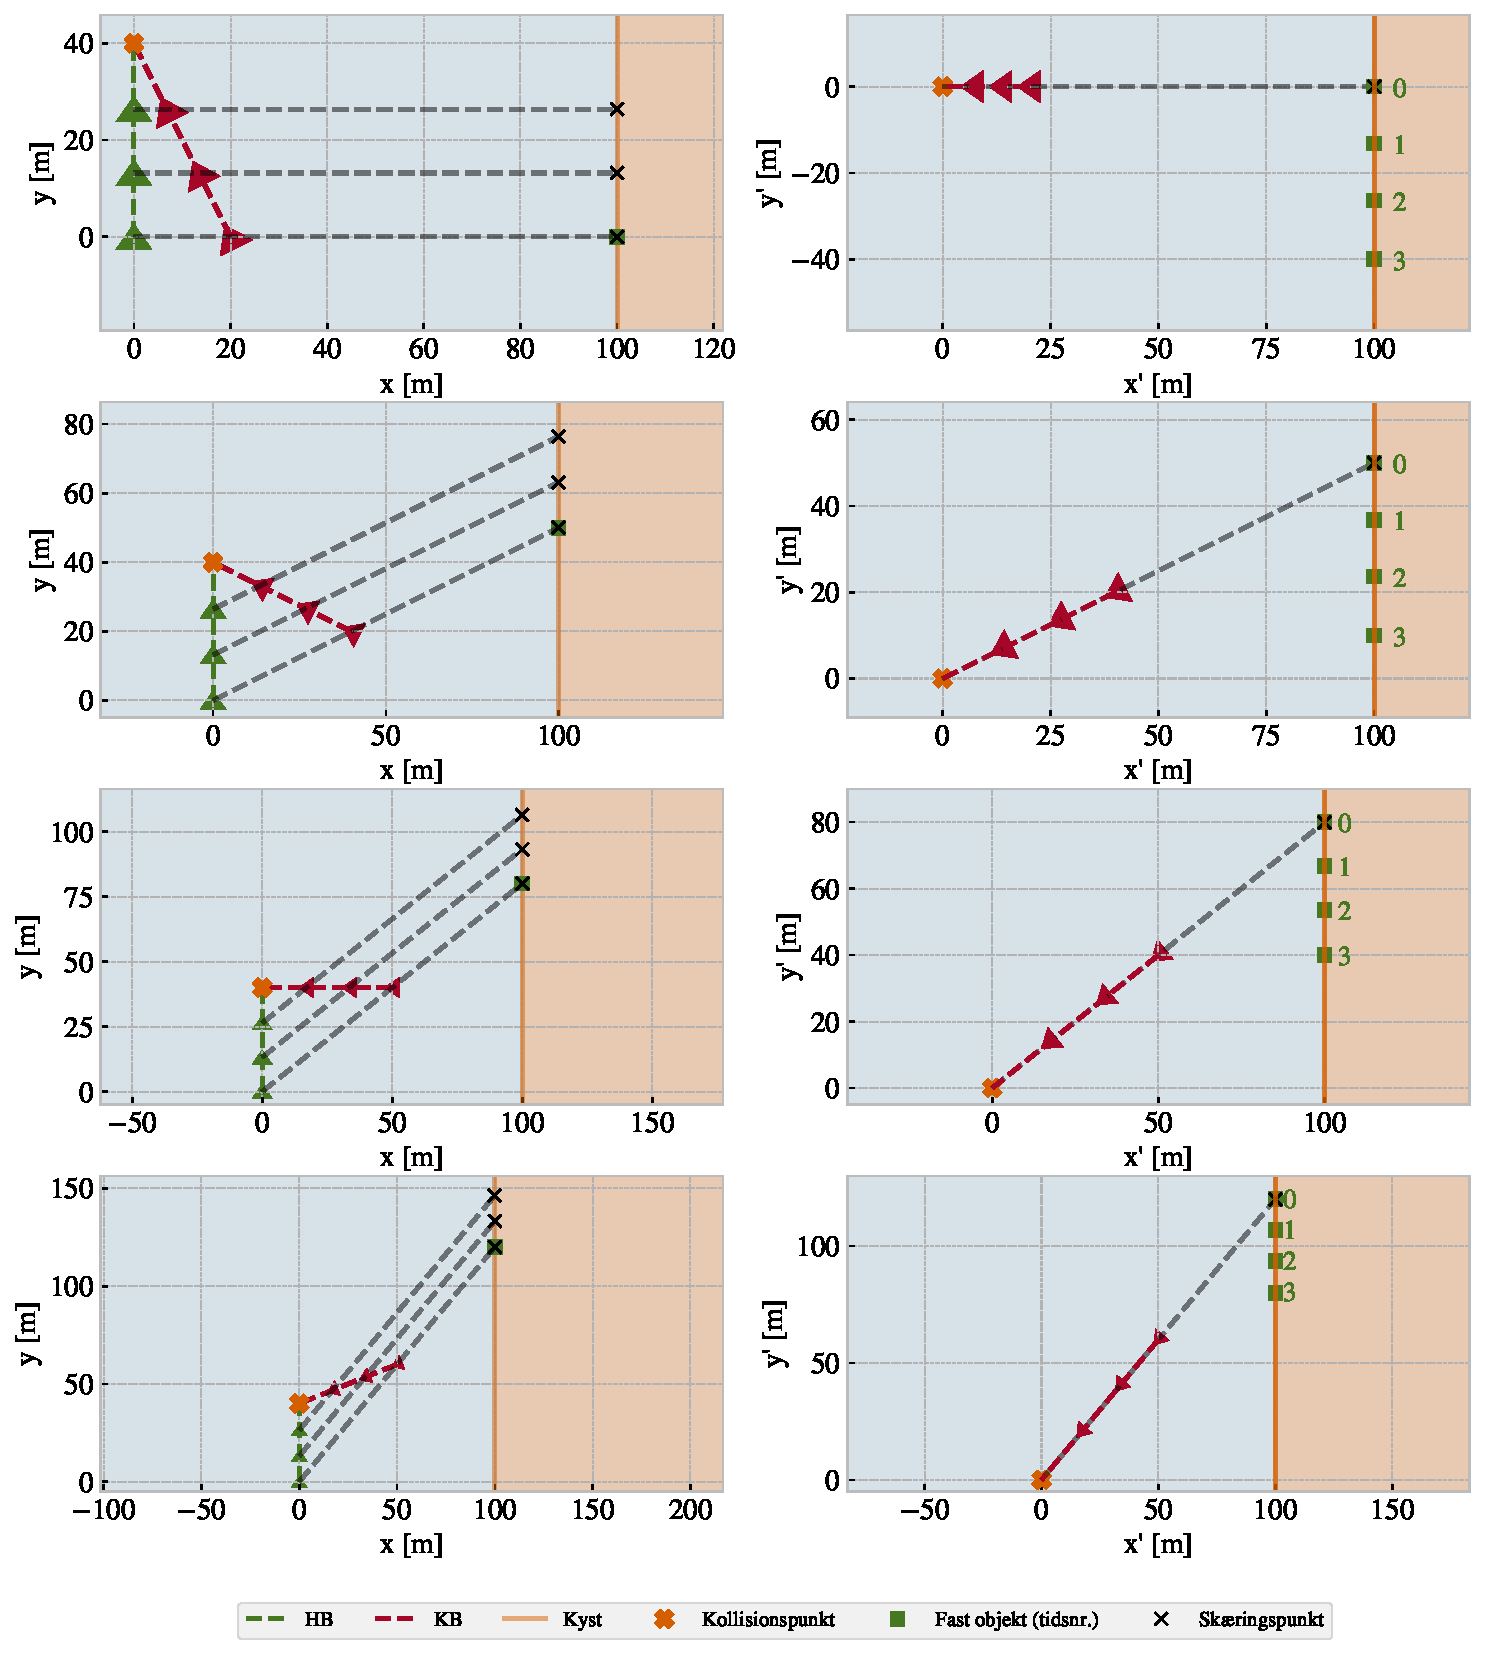
\includegraphics[width=\linewidth]{figures/subplot_C1.pdf}
  \caption[A table inside a caption]{
\begin{tabular}{|c|c|c|c|c|}
\hline
Figurrække & $HB_{start}$  & $KB_{start}$ & $HB_{slut}$ & $KB_{slut}$\\ \hline
1  & (0,0) & (20,0) & (0, 40) & (0, 40) \\ \hline
2  & (0,0) & (40,30) & (0, 40) & (0, 40) \\ \hline
3  & (0,0) & (50,40) & (0, 40) & (0, 40) \\ \hline
4  & (0,0) & (50,60) & (0, 40) & (0, 40) \\ \hline
\end{tabular}}
  \label{fig:subplot_C1}
\end{figure}

\begin{figure}[H]
  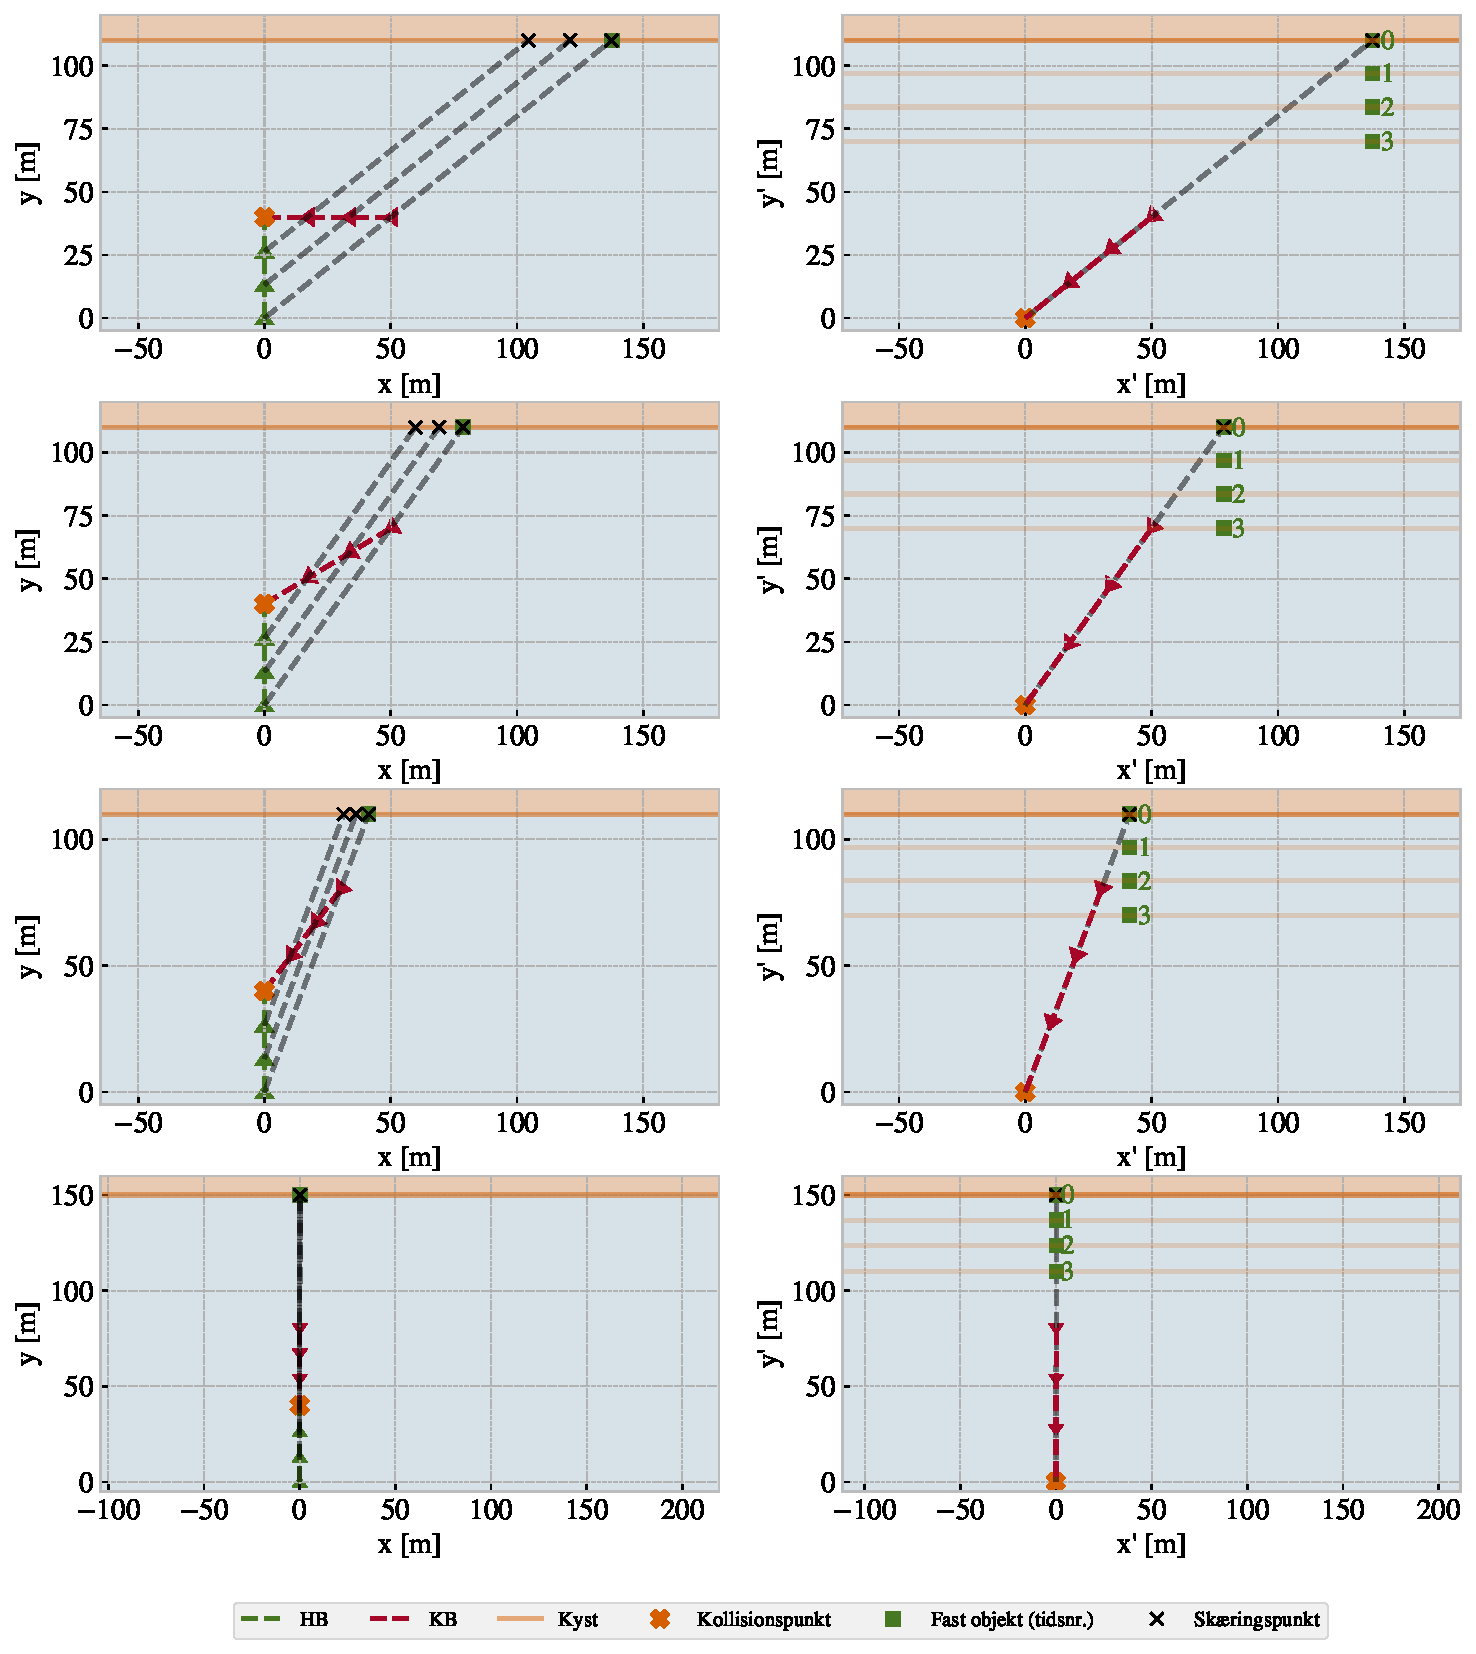
\includegraphics[width=\linewidth]{figures/subplot_C2.pdf}
  \caption[A table inside a caption]{
\begin{tabular}{|c|c|c|c|c|}
\hline
Figurrække & $HB_{start}$  & $KB_{start}$ & $HB_{slut}$ & $KB_{slut}$\\ \hline
1  & (0,0) & (50,40) & (0, 40) & (0, 40) \\ \hline
2  & (0,0) & (50,70) & (0, 40) & (0, 40) \\ \hline
3  & (0,0) & (30,80) & (0, 40) & (0, 40) \\ \hline
4  & (0,0) & (0.1,80) & (0, 40) & (0, 40) \\ \hline
\end{tabular}}
  \label{fig:subplot_C2}
\end{figure}


\clearpage
\subsection{Simmuleringer uden kollision}
\begin{figure}[H]
  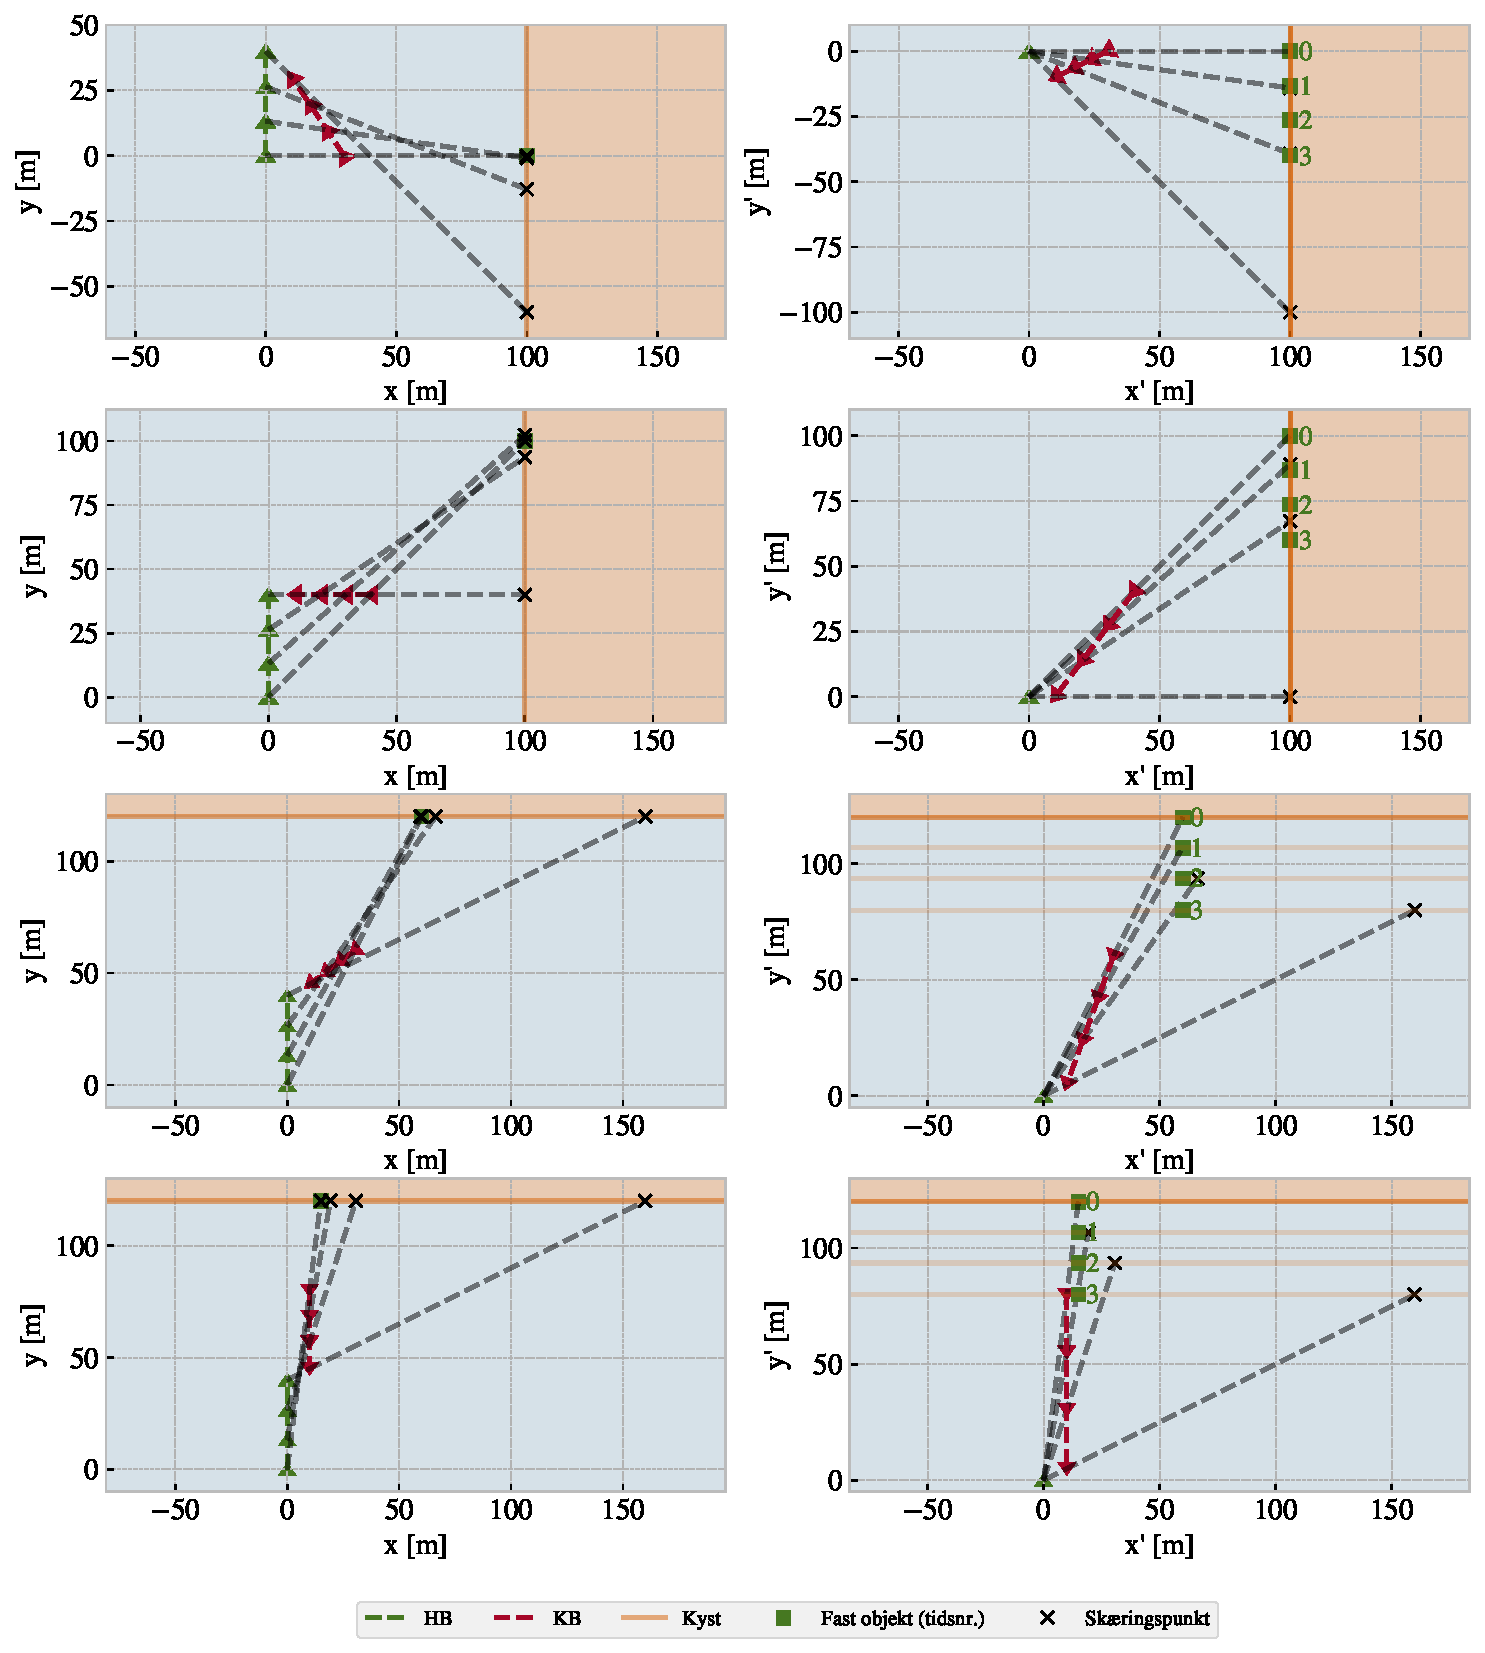
\includegraphics[width=\linewidth]{figures/subplot_NC1.pdf}
  \caption[A table inside a caption]{
\begin{tabular}{|c|c|c|c|c|}
\hline
Figurrække & $HB_{start}$  & $KB_{start}$ & $HB_{slut}$ & $KB_{slut}$\\ \hline
1  & (0,0) & (30,0) & (0, 40) & (10, 30) \\ \hline
2  & (0,0) & (40,40) & (0, 40) & (10, 40) \\ \hline
3  & (0,0) & (30,60) & (0, 40) & (10, 44) \\ \hline
4  & (0,0) & (10,80) & (0, 40) & (10, 44) \\ \hline
\end{tabular}}
  \label{fig:subplot_NC1}
\end{figure}








\end{document}
